\section{Project Assessment}
\begin{figure}[h]
    \centering
    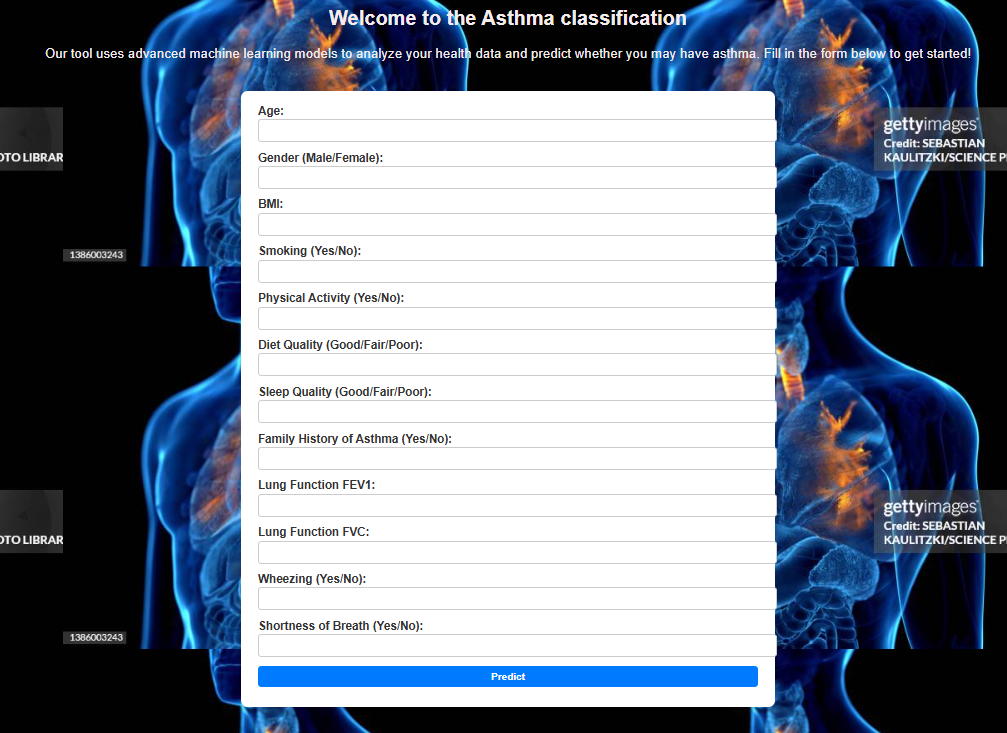
\includegraphics[width=0.9\linewidth]{Images/u1.png}
    \caption{Home Page}
    \label{fig:ui1}
\end{figure}
The asthma prediction tool starts on the Input Page, where users must enter their health-related data. Among the information in this data that helps the model understand the user's general health profile are age, gender, and BMI. Other factors, such smoking status and physical activity levels, are included since they may have an impact on respiratory health. The questionnaire also gathers information on food and sleep quality, both of which have been linked to overall lung health. The asthma prediction tool starts on the Input Page, where users must enter their health-related data. Among the information in this data that helps the model understand the user's general health profile are age, gender, and BMI. Other factors, such smoking status and physical activity levels, are included since they may have an impact on respiratory health. The questionnaire also gathers information on food and sleep quality, both of which have been linked to overall lung health. 
\begin{figure}[h]
    \centering
    \begin{minipage}{0.5\linewidth}
        \centering
        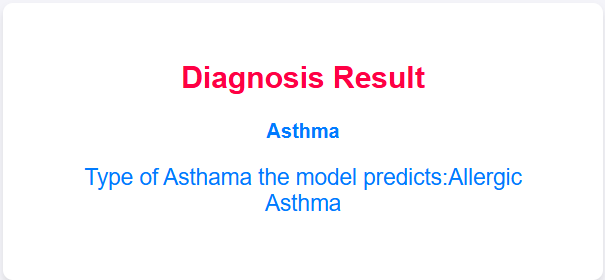
\includegraphics[width=\linewidth]{Images/u2.png}
        \caption{Allergic Asthma}
        \label{fig:ui5}
    \end{minipage}
\end{figure}
\newline
As Figure 4.2 shows that the diagnosis result indicates Asthma, specifically the type predicted by the model is Allergic Asthma.
\begin{figure}[h]
    \centering
    \begin{minipage}{0.5\linewidth}
        \centering
        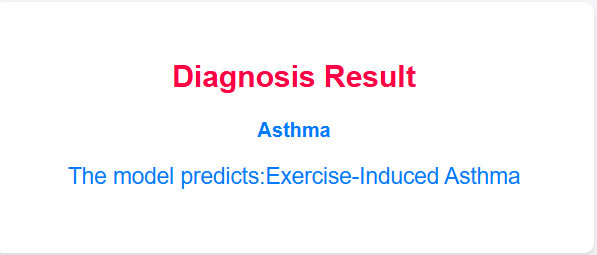
\includegraphics[width=\linewidth]{Images/u3.png}
        \caption{Exercise-Induced Asthma}
        \label{fig:ui5}
    \end{minipage}
\end{figure}
\newline 
As Figure 4.3 shows that the diagnosis result indicates Asthma, with the model predicting Exercise-Induced Asthma.
\begin{figure}[h]
    \centering
    \begin{minipage}{0.5\linewidth}
        \centering
        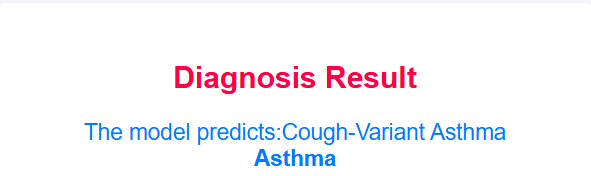
\includegraphics[width=\linewidth]{Images/u4.png}
        \caption{Cough-Variant Asthma}
        \label{fig:ui5}
    \end{minipage}
\end{figure}
\newline 
As Figure 4.4 shows that the diagnosis result indicates Asthma, and the model predicts the subtype as Cough-Variant Asthma.

\section{Personal Development}
The classification of asthma diseases was the main emphasis of the internship. By promoting technical proficiency, strengthening problem-solving abilities, and developing critical soft skills, machine learning greatly aided in human growth. Hands-on expertise with a variety of techniques, such as Support Vector Machines, Random Forest, and Logistic Regression, was made possible by participating in real-world machine learning projects. Additionally, this work involved statistical analysis, feature engineering, and advanced data preprocessing, which strengthened mastery of tools like Pandas, NumPy, and Scikit-learn. Working with frameworks like Flask also made it possible to create web-based apps for implementing machine learning models, which helped to close the gap between theory and practice.

Through challenges including managing inconsistent data, maximizing model performance, and guaranteeing system scalability, the internship honed problem-solving abilities. The exercise highlighted the need of analytical thinking and flexibility in practical situations by critically analyzing several algorithms and choosing the best one for classifying asthma.

Collaboration and time management were essential components of this experience. While regular interactions with mentors and team members enhanced collaboration and teamwork, juggling multiple tasks under short deadlines sharpened organizational skills. Additionally, communicating findings in an understandable manner through reports and visualizations improved communication skills and made complicated information understandable to both technical and non-technical audiences.
\section{Skills Consolidation}
Through weekly tasks and learning opportunities, skill in data processing, model building, and system integration rapidly developed, and significant knowledge of software development methodologies, machine learning, and artificial intelligence was acquired throughout the internship.
\begin{table}[h]
    \centering
    \caption{Week-wise Work Progress}
    \begin{center}  
        \begin{tabular}{|c|p{12.4cm}|}
            \hline
            \textbf{Week} & \textbf{Work Progress} \\ \hline
            1 &Identified the issue statement, gathered requirements, and set project objectives. Conducted a feasibility analysis to finalize the scope. \\ \hline
            2 & gathered a variety of datasets from different sources and conducted preliminary research to comprehend their structure and possible problems. \\ \hline
            3 & Datasets were cleaned, preprocessed, and divided into subsets for testing, validation, and training. Missing values and inconsistencies were fixed, and data was normalized for consistency. \\ \hline
            4 & Designed and trained the machine learning model, fine-tuning its architecture to optimize performance based on project requirements. \\ \hline
            5 & Integrated the ML model into a web application using Flask for the backend and HTML/CSS for the front end. Conducted extensive system testing to identify and resolve bugs.\\ \hline
            6 & Deployed the application, collected user feedback, and implemented final optimizations. Completed documentation and prepared the final project report. \\ \hline
        \end{tabular}
    \end{center}
    \label{tab:work}
\end{table}
\section{Conclusion}
From understanding the project objectives to putting a functional application into practice, every stage of the internship provided new insights and chances to learn new skills. Accuracy and adaptability are crucial in real-world scenarios, as demonstrated by the systematic approach to problem-solving that involved data pretreatment, model training, and system integration.\\
The final result, a successfully deployed AI/ML system, demonstrated how theoretical understanding might be applied to practical issues. It also underlined how important critical thinking, cooperation, and lifelong learning are to achieving project objectives. This internship not only improved technical skills but also promoted a deeper understanding of the complexities and potential applications of AI/ML technology in solving contemporary problems.
